\documentclass{scrartcl}
\usepackage[utf8]{inputenc}
\usepackage[T1]{fontenc}      
\usepackage[francais]{babel}
\usepackage{algorithm2e}
% Layout and figures
\usepackage[top=2.5cm,bottom=2.5cm,right=2.5cm,left=2.5cm]{geometry}
% Links
\usepackage{url}
\usepackage{hyperref}
\hypersetup{
    colorlinks,
    citecolor=black,
    filecolor=black,
    linkcolor=black,
    urlcolor=black
}

% New commands
\newcommand{\annexe}{\part{Annexes}\appendix}
\newcommand{\biblio}[1]{\bibliographystyle{plain}\bibliography{#1}\nocite{*}}

\newcommand{\doctitle}[1]{
	\title{LINGI1121 - Algorithmique et structure de données}
	\subtitle{#1}
	\author{\textbf{Groupe 9}\\
	\textsc{Aghakhani} Ghazaleh (1161-11-00)\\
	\textsc{Carlier} Alexandre (5042-13-00)\\
	\textsc{Cleeremans} Tanguy ()\\
	\textsc{Paris} Antoine (3158-13-00)\\
	\textsc{Prie\"{e}ls} Antoine (3290-13-00)}\\
	\textsc{Stévenart Meeus} Florian (6273-13-00)}
	\date{\today}

	\begin{document}

	\maketitle
	%\tableofcontents
}
\doctitle{Mission 1 : piles, files, listes chaînées}
\lstset{language={Java}}
\lstset{
  numbers=left,
  numberstyle=\tiny\color{gray},
  basicstyle=\textrm\small\ttfamily,
  keywordstyle=\bfseries\color{black},
  frame=single,
  commentstyle=\color{gray}=small,
  stringstyle=\color{dkgreen},
  %backgroundcolor=\color{gray!10},
  %tabsize=2,
  rulecolor=\color{black},
  %title=\lstname,
  breaklines=true,
  framextopmargin=2pt,
  framexbottommargin=2pt,
  extendedchars=true,
}

\section{Réponses aux questions}
\begin{enumerate}
	\item Un type abstrait est une spécification
	d'un ensemble de données et de l'ensemble des
	opérations qu'on peut lui appliquer (sans se
	préoccuper de l'implémentation de celles-ci).
	Il s'agit en quelque sorte d'un cahier des
	charges pour une structure de données.
	\cite{wiki-tad}\cite{mod-obj}
	
	Quant au choix d'utiliser une classe ou une
	interface en Java pour décrire un type abstrait
	de données, il semble tout indiqué. Une interface
	Java n'a pour but que de définir une implémentation ;
	elle est par définition abstraite et ne fixe aucun
	aspect de l'implémentation.\cite{nino} Cela colle
	parfaitement à la définition de type abstrait de
	données.
	\item L'opération \lstinline{push} pour une pile
	implémentée à l'aide d'une liste s'implémente en
	parcourant toute la liste jusqu'à arriver à la fin
	de la liste. \`{A} ce moment là, on modifie le
	pointeur vers l'élément suivant du dernier élement
	pour le faire pointer vers le nouvel élément.
	
	L'opération \lstinline{pop} s'implément à peu près
	de la même façon. On parcourt la liste jusqu'à
	arriver à la fin. \`{A} ce moment là, on retourne
	le dernier élément de la liste et on modifie le
	pointeur de l'avant-dernier élément pour le faire
	pointer vers \lstinline{null}.
	
	Cette implémentation n'est pas efficace parce qu'il
	faut parcourir toute la liste à chaque opération, ce
	qui peut vite devenir gênant pour des listes contenant
	des millions d'éléments...
	\item L'implémentation d'une pile par la classe
	\lstinline{java.util.Stack} fournit 5
	fonctions :
	\begin{itemize}
		\item \lstinline{boolean empty()} :
		teste si la pile est vide ;	
		\item \lstinline{E peek()} : retourne
		l'objet au sommet de la pile sans l'enlever ;
		\item \lstinline{E pop()} : retourne
		l'objet au sommet de la pile en l'enlevant ;
		\item \lstinline{E push(E item)} :
		ajoute un élément au sommet de la pile ;
		\item \lstinline{int search(Object o)} :
		retourne la position de l'objet dans la pile.
	\end{itemize}
	
	En regardant le code source de cette classe, on
	constate que la plupart des fonctions sont héritées
	de la classe \lstinline{Vector<E>}. En
	allant ensuite regarder le code source de cette classe,
	on se rend compte que celle-ci utilise un tableau pour
	stocker des éléments ainsi qu'un compteur d'éléments. 
	Cela signifie donc qu'en Java, les éléments d'une liste
	chaînée sont stockés dans un tableau. Cette solution
	est beaucoup plus efficace que celle proprosé à la
	question précédente puisqu'il est possible d'accèder au
	dernier élément de la liste sans la parcourir entièrement.
	\item La méthode la plus efficace pour implémenter
	une pile avec deux files provient de \cite{stack1}.
	Soient deux piles $A$ et $B$. $A$ contient les
	éléments au sommet de la pile tandis que $B$
	contient les éléments du bas de la pile. La taille
	de $A$ doit toujours être inférieur à la
	racine carrée de la taille de $B$.
	
	\lstinline{push} s'effectue simplement
	en effectuant \lstinline{enqueue} 
	du nouvel élément sur la pile $A$ et ensuite en
	effectuant \lstinline{dequeue} puis
	\lstinline{enqueue} sur tous les autres
	élément de $A$. De cette manière le nouvel élément
	est bien le premier élément de $A$.
	
	Si le nombre d'élément contenu dans $A$ devient
	plus grand que la racine carrée du nombre
	d'élément contenu dans $B$, on
	\lstinline{enqueue} tous les éléments
	de $B$ sur $A$ un par un et on inverse $A$ et $B$.
	
	Enfin, \lstinline{pop} s'effectue en
	effectuant \lstinline{dequeue} sur $A$
	et en retournant le résultat si $A$ n'est pas vide
	et en effectuant \lstinline{dequeue}
	sur $B$ dans le cas contraire.
	
	En terme de complexité,
	\lstinline{pop} s'effectue en
	$\mathcal{O}(1)$.
	
	Pour \lstinline{push}, deux cas sont
	à analyser. Dans le premier cas,
	$|A| < \sqrt{|B|}$ et on a donc
	$\mathcal{O}(\sqrt{n})$. Dans le cas contraire,
	\lstinline{push}\ s'effectue en
	$\mathcal{O}(n)$ mais après cela, $A$ est vide et
	il faudra un temps $\mathcal{O}(\sqrt{n})$ avant
	que ce cas ne se reproduise, le coût amorti est
	donc en $\mathcal{O}(\sqrt{n})$.
	\item
	\item
	\item
	\item Un itérateur permet de parcourir une collection
        d'objets élément par élément. L'implémentation des
        itérateurs est très générique puisque ceux-ci peuvent
        être utilisés de la même manière sur n'importe quel
        type de structure de données.
	
	La modification des données par l'itérateur lui-même
        (en faisant appel à sa méthode \lstinline{remove}) ne posera pas
        de souci. Cependant, la modification concurrente de
        la collection par un autre thread pourrait poser problème.
        En effet, un élément pourrait être renvoyé deux fois ou
        l'itérateur pourrait sauter un élément de la liste sans
        le renvoyer. C'est pourquoi la classe \lstinline{Iterator} doir lancer
        une \lstinline{ConcurrentModificationException} si n'importe quel élément
        de la collection a été modifié ou supprimé par une autre
        méthode que la sienne.\cite{iter-openclass}
	 
	Il est possible d'empêcher la modification de la liste en
        ajoutant un booléen en tant que variable globale. Lors de
        l'initialisation de l'itérateur, ce booléen serait mis à
        \lstinline{false} et chaque appel à
        \lstinline{push} ou \lstinline{pop}
        ferait passer cette variable à \lstinline{true}.
        Ainsi, lors de la progression de l'itérateur une vérification
        de la variable permettra de déterminer si la pile a été modifiée.
        L'implémentation aura alors une forme semblable à la
        suivante\footnote{Seules les lignes 3, 15, 28, 37 et 48 ont
        été modifiées. Le reste provient directement du code source.}.
	 
	\definecolor{gray}{rgb}{0.75,0.75,0.75}
	\definecolor{dkgreen}{rgb}{0,0.6,0}
	\begin{lstlisting}[language=Java]
public class Stack<Item> implements Iterable<Item> {
	 
    private boolean modified = true;
    //Les autres variables restent inchangees
	 
    /**
    * Add the item to the stack.
    */
    public void push(Item item) {
        Node oldfirst = first;
        first = new Node();
        first.item = item;
        first.next = oldfirst;
        N++;
        modified = true;
    }
	 
    /**
    * Delete and return the item most recently added to the stack.
    * Throw an exception if no such item exists because the stack is empty.
    */
    public Item pop() {
        if (isEmpty()) throw new RuntimeException("Stack underflow");
        Item item = first.item;        // save item to return
        first = first.next;            // delete first node
        N--;
        return item;                   // return the saved item
        modified = true;
    }
    
    /**
    * Return an iterator to the stack that iterates through the 
    * items in LIFO order.
    */
    public Iterator<Item> iterator()  { 
    	return new ListIterator();
    	modified = false;
    }

    // an iterator, doesn't implement remove() since it's optional
    private class ListIterator implements Iterator<Item> {
        private Node current = first;
        public boolean hasNext() { return current != null; }
        public void remove() { throw new UnsupportedOperationException(); }

        public Item next() {
            if (!hasNext()) throw new NoSuchElementException();
            if (modified) throw new ConcurrentModificationException();
            Item item = current.item;
            current = current.next; 
            return item;
        }
    }
    
    //Le reste du code n'est pas modifie
	 
	 }
	 \end{lstlisting}
	 \vspace{0.5cm}
	 
        Laisser la méthode \lstinline{remove()} vide
        ne poserait pas de problème lors de la compilation ou
        l'exécution du code. Cependant, il ne faut surtout pas
        oublier que cette méthode est vide car si le programme
        utilise cette méthode, aucun élément ne sera retiré de
        la liste. Après une rapide recherche du code source de
        la classe \lstinline{Stack}, nous avons pu remarquer que pour remédier
        à cela, la méthode n'est pas vide mais une
        \lstinline{UnsupportedOperationException} est lancée.
	 
	\item La notation tilde est définie comme étant\cite{tilde-pdf}
        $$g(N) \sim a * f(N) \quad avec \quad \lim\limits_{N
        \longrightarrow +\infty} \frac{g(N)}{f(N)} = a$$

	Comparons la notation $\sim$ aux autres notations que
        nous avons utilisé précédemment pour mesurer la complexité
        de fonctions :
	$\Omega(f(N))$, $\mathcal{O}(f(N))$ et $\Theta(f(N))$.
	Ces notations se différencient en deux grands types :
        $\mathcal{O}$ et $\Omega$ nous fournissent des bornes
        respectivement inférieure et supérieure tandis que $\sim$
        et $\Theta$ nous donnent un ordre de grandeur quant à la
        complexité d'exécution d'un algorithme.
	Les deux notations les plus pratiques sont les notations
        $\mathcal{O}$ et $\sim$. Cependant, alors que $\mathcal{O}$
        nous donne simplement une borne supérieure (ce qui est utile
        pour nous donner une idée générale de ce qui pourrait arriver
        dans le pire des cas), $\sim$ nous permet de définir aussi une
        borne inférieure. De plus, cette dernière conserve le coefficient
        du terme de plus haut degré et nous trouvons donc une précision
        plus grande pour les tableaux de très grande taille
        (cfr. Figure~\ref{fig:complex_tilde}).

        \begin{figure}[ht]
                \centering
	        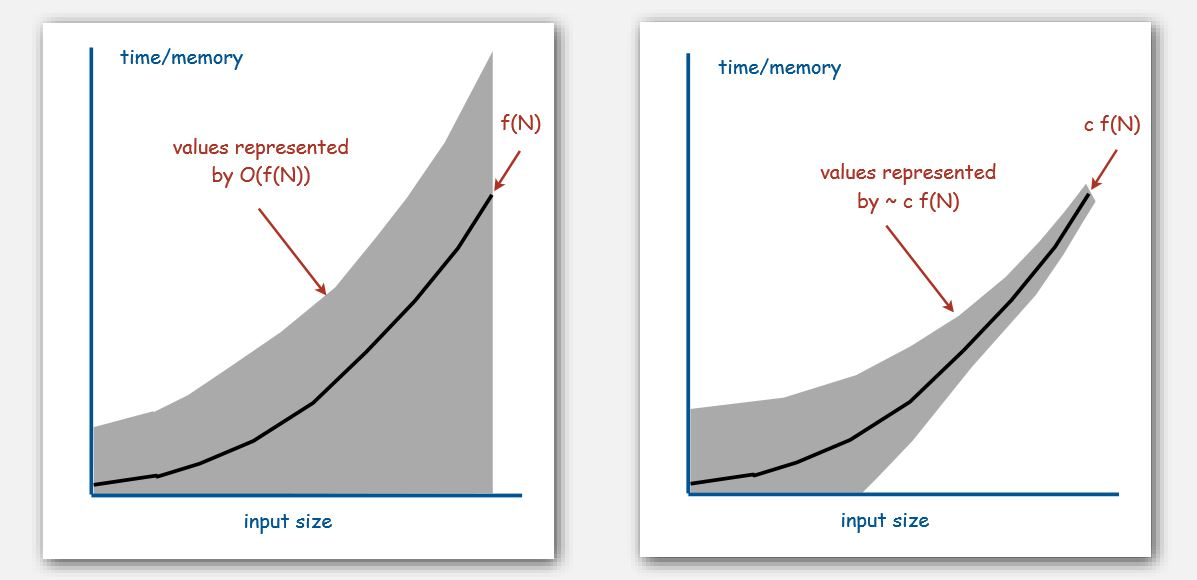
\includegraphics[width=0.8\textwidth]{complex_tilde.jpg}
	        \caption{Comparaison de la précision des notations
                $\mathcal{O}$ et $\sim$~\cite{image-complex}.}
	        \label{fig:complex_tilde}
        \end{figure}	

	\item
	\item
\end{enumerate}

\bibliographystyle{plain}
\bibliography{./biblio}

\end{document}
